\documentclass[a4paper,12pt]{article}
\title{Anleitung für ZM1000 Nixi Uhr}

\usepackage{graphicx}
\usepackage{subcaption}

\usepackage{xcolor,colortbl}

\newcommand{\mc}[2]{\multicolumn{#1}{c}{#2}}
\definecolor{Gray}{gray}{0.85}
\definecolor{LightCyan}{rgb}{0.88,1,1}

\newcolumntype{a}{>{\columncolor{Gray}}c}
\newcolumntype{b}{>{\columncolor{white}}c}

\begin{document}
\maketitle

\begin{figure}[h!]
    \centering
    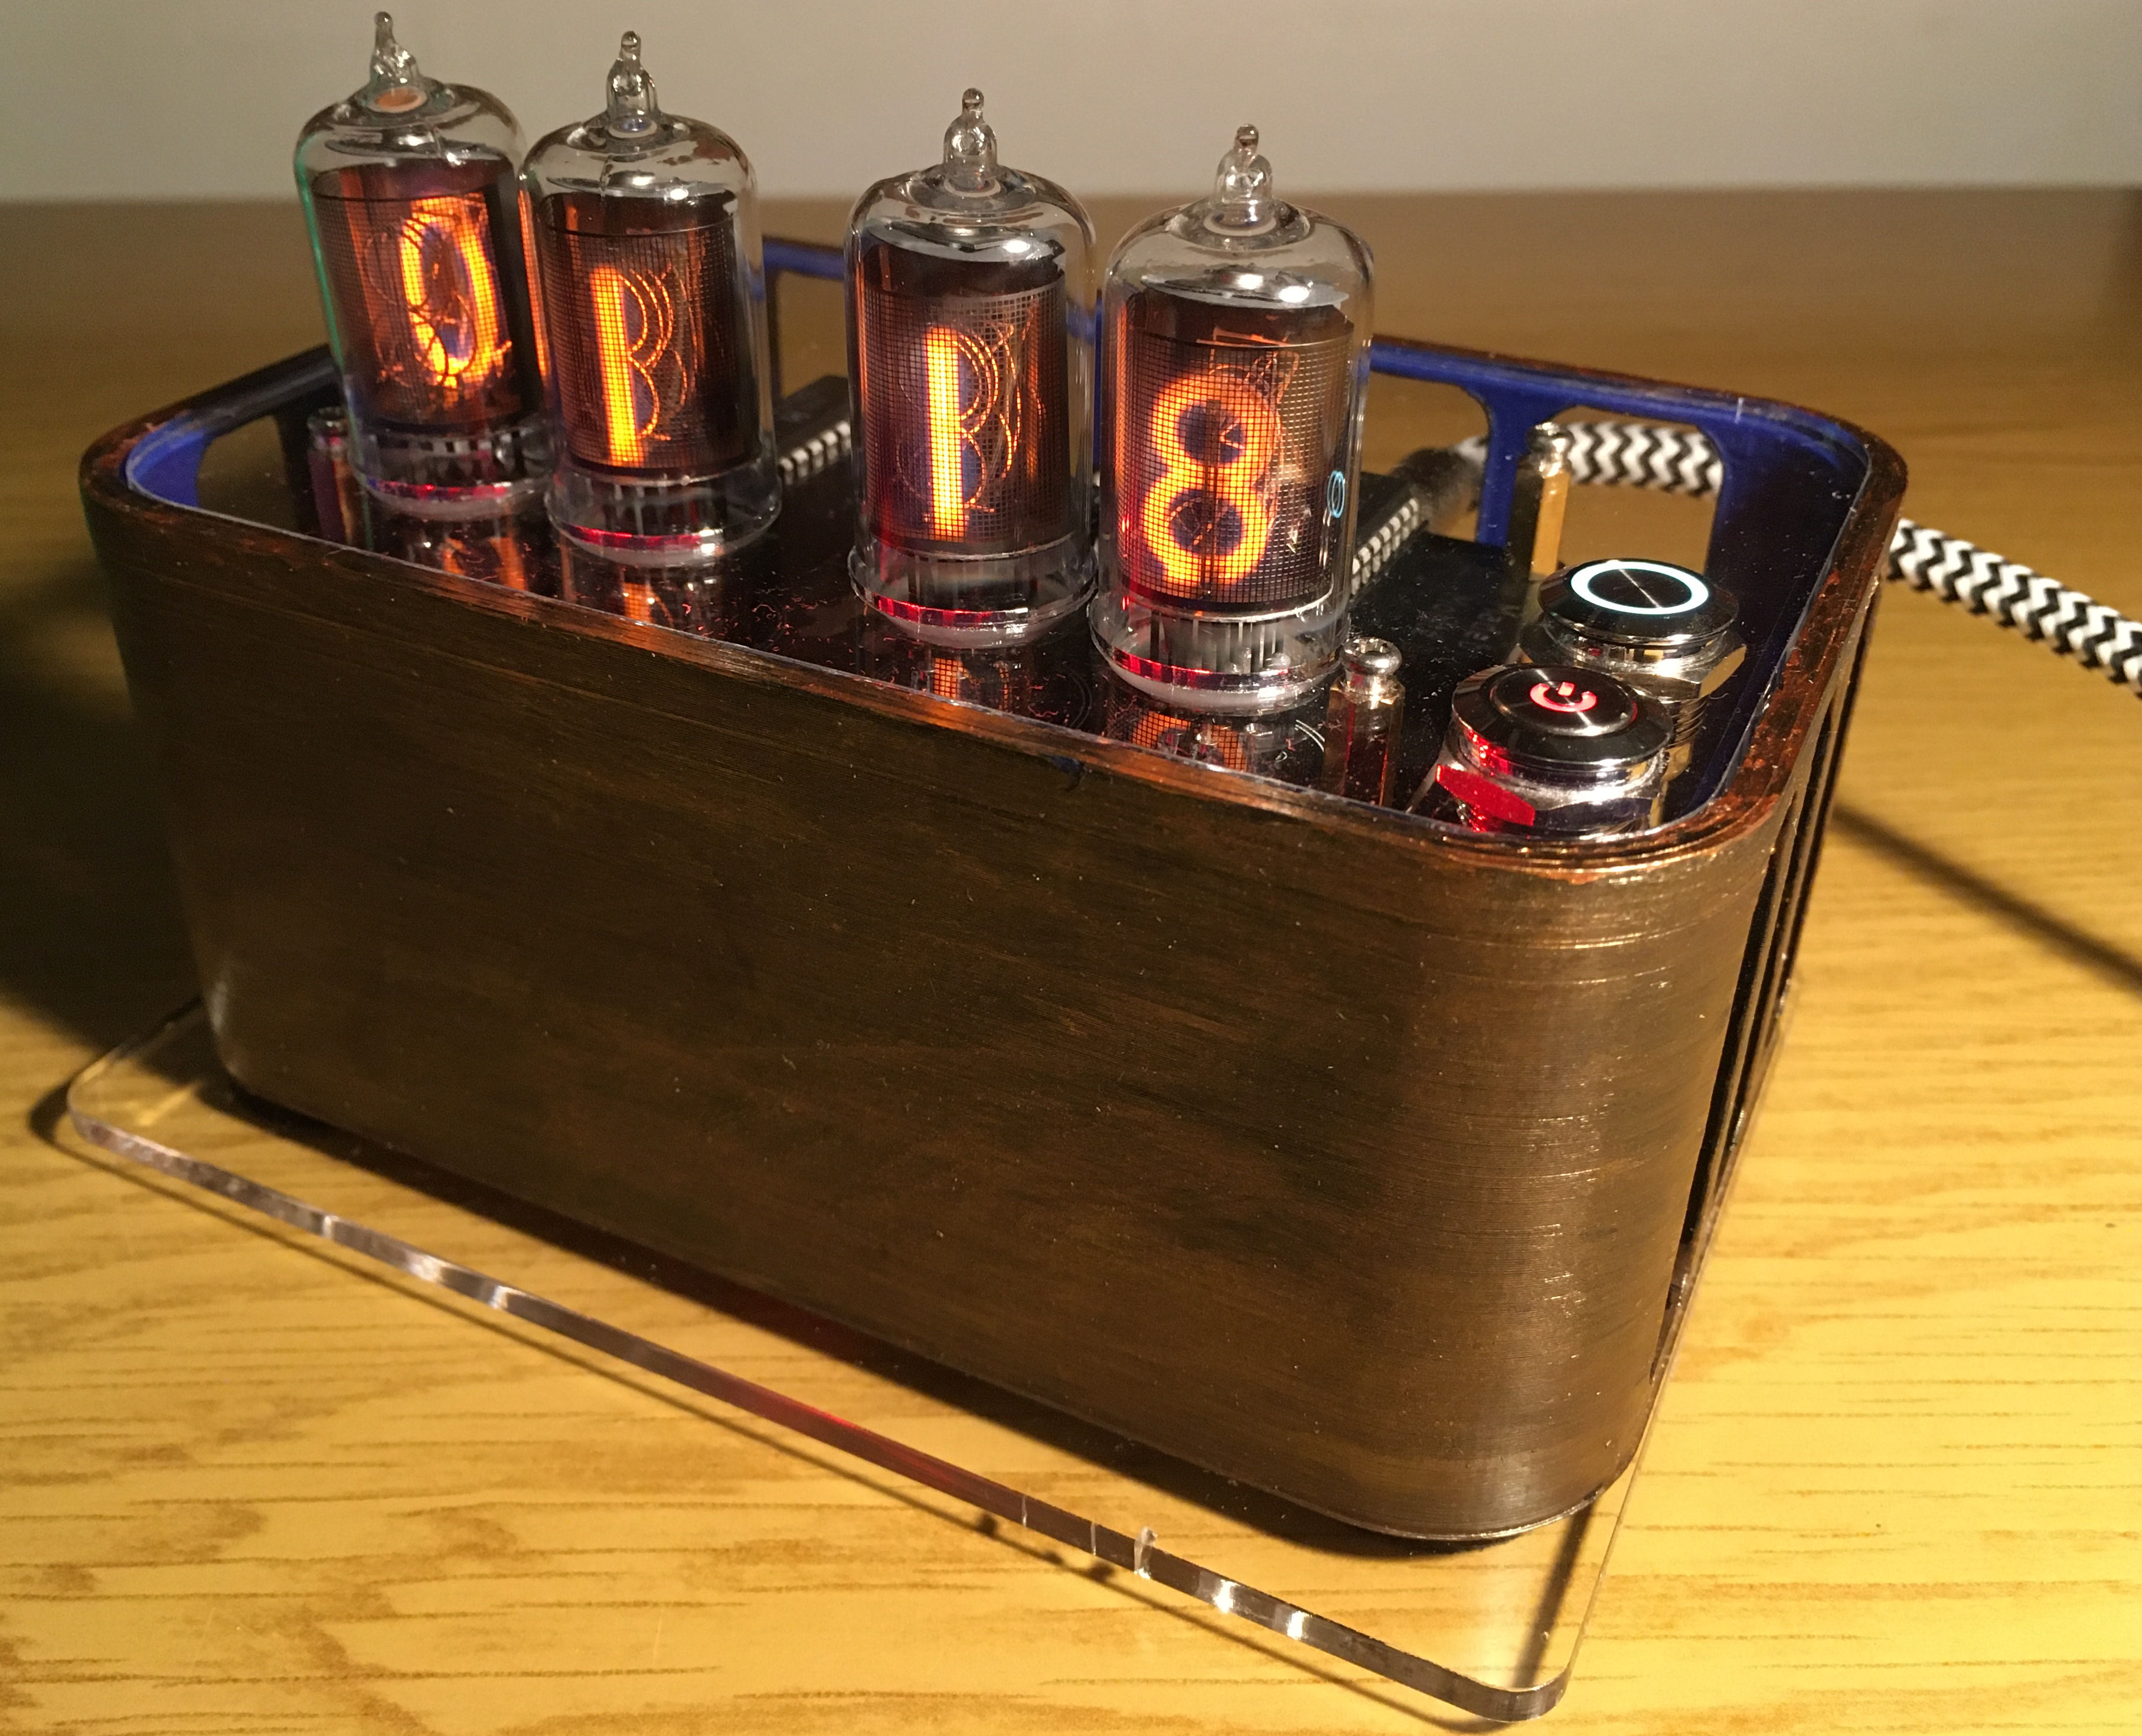
\includegraphics[width=1\textwidth]{Clock.jpg}
\end{figure}

\newpage

\section{Einleitung}

Die Uhr hat einen \textbf{Power Button} und einen \textbf{Funktions Button} beide sind auf der rechten Seite (von vorne gesehen) auf der Uhr zu finden.

\begin{figure}[h!]
    \centering
    \begin{subfigure}[b]{0.1\textwidth}
        
\includegraphics[width=\textwidth]{Power_BTN.png}
    \end{subfigure}
    ~ %add desired spacing between images, e. g. ~, \quad, \qquad, \hfill etc. 
      %(or a blank line to force the subfigure onto a new line)
    \begin{subfigure}[b]{0.1\textwidth}
        
\includegraphics[width=\textwidth]{Push_BTN.png}
    \end{subfigure}
\end{figure}

\section{Funktion}

\begin{tabular}[h]{|a|b|a|b|}
    \hline
    \rowcolor{LightCyan}
    Knopf & Funktion & Druckdauer & Kommentar \\
    \hline
    
\includegraphics[0.08\textwidth]{Power_BTN.png} & standby & kurz& Beenden durch erneutes drücken\\
    \hline
    
\includegraphics[0.08\textwidth]{Push_BTN.png} & Temp. und Luftf. & kurz & Automatisches beenden \\
    \hline
    
\includegraphics[0.08\textwidth]{Push_BTN.png} & Stoppuhr &lang& Beenden durch drücken des Power Button\\
    \hline
\end{tabular}

\section{Internetverbindung}

Ist die verbinfung zum INternet gegeben wird bei der Anzeige der Temperatur und Luftfeuchtigkeit bei den letzten beiden Ziffern die Aussentemperatur angezeigt.
  
\end{document}